%%%%%%%%%%%%%%%%%%%%%%%%%%%%%%%%%%%%%%%%%%%%%%%%%%%%%%%%%%%%%%%%%%%%%%%%%%%%%%%%%%
\begin{frame}[fragile]\frametitle{}

\begin{center}
{\Large Introduction to spaCy}
\end{center}
\end{frame}
%

%%%%%%%%%%%%%%%%%%%%%%%%%%%%%%%%%%%%%%%%%%%%%%%%%%%%%%%%%%%%%%%%%%%%%%%%%%%%%%%%%%
\begin{frame}[fragile]\frametitle{What is spaCy?}
  \begin{itemize}
    \item spaCy is a free, open-source library for advanced Natural Language Processing (NLP) in Python.
		\item Production ready.
		\item Used to build information extraction or natural language understanding systems, or to pre-process text for deep learning.
  \end{itemize}
	
{\tiny (Ref: https://spacy.io/usage/spacy-101)}
\end{frame}



%%%%%%%%%%%%%%%%%%%%%%%%%%%%%%%%%%%%%%%%%%%%%%%%%%%%%%%%%%%%%%%%%%%%%%%%%%%%%%%%%%
\begin{frame}[fragile]\frametitle{What spaCy isn't?}
  \begin{itemize}
    \item Not a platform or “an API” or software as a service, or a web application
		\item Not an out-of-the-box chat bot engine.
		\item Not research software.  It’s built on the latest research, but it’s designed to get things done.
		\item Not a company. It’s an open-source library. Company's name is `Explosion AI'.
  \end{itemize}
	
{\tiny (Ref: https://spacy.io/usage/spacy-101)}
\end{frame}

%%%%%%%%%%%%%%%%%%%%%%%%%%%%%%%%%%%%%%%%%%%%%%%%%%%%%%%%%%%%%%%%%%%%%%%%%%%%%%%%%%
\begin{frame}[fragile]\frametitle{Installation}
Based on OS, version, etc an installation command can be generated at https://spacy.io/usage

	
\begin{center}
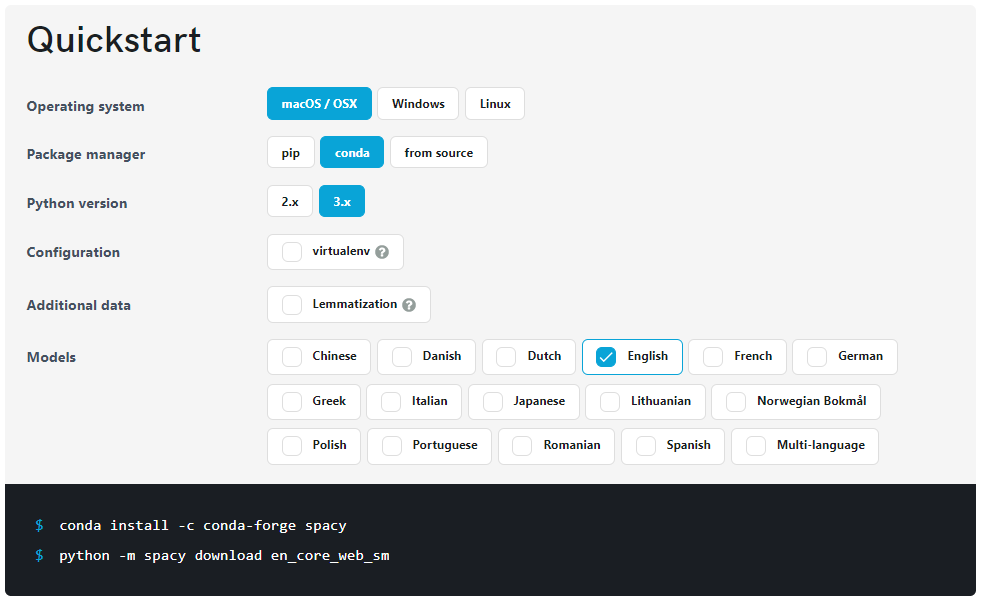
\includegraphics[width=0.8\linewidth,keepaspectratio]{spacy3}
\end{center}

{\tiny (Ref: https://spacy.io/usage/spacy-101)}
\end{frame}

%%%%%%%%%%%%%%%%%%%%%%%%%%%%%%%%%%%%%%%%%%%%%%%%%%%%%%%%%%%%%%%%%%%%%%%%%%%%%%%%%%
\begin{frame}[fragile]\frametitle{Features}
\begin{center}
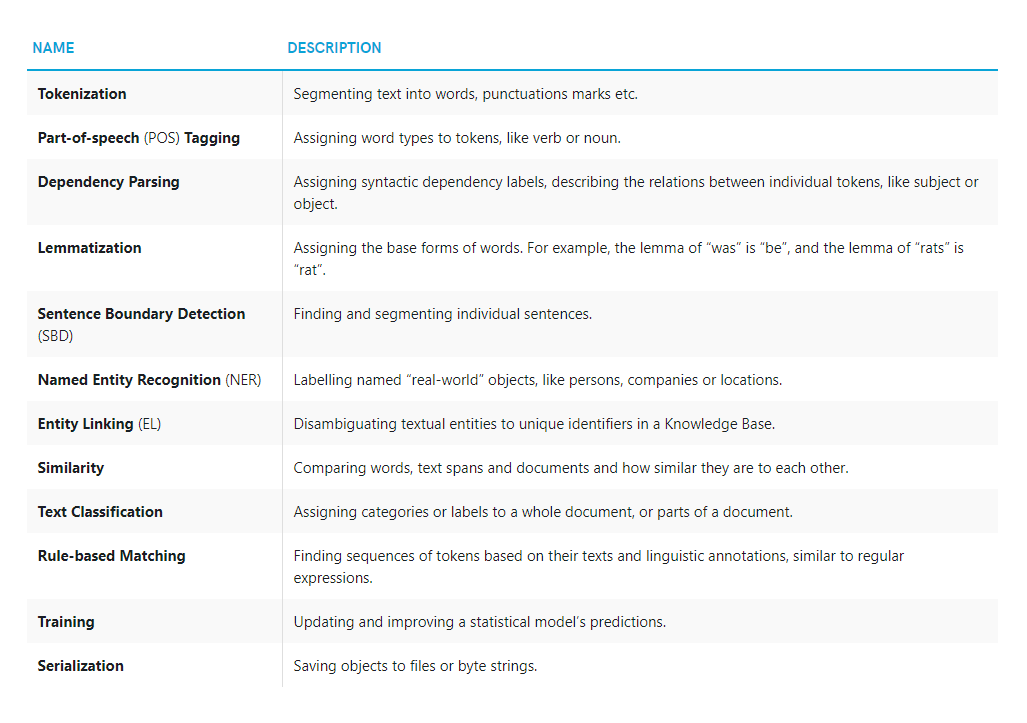
\includegraphics[width=0.8\linewidth,keepaspectratio]{spacy4}
\end{center}

{\tiny (Ref: https://spacy.io/usage/spacy-101)}
\end{frame}



%%%%%%%%%%%%%%%%%%%%%%%%%%%%%%%%%%%%%%%%%%%%%%%%%%%%%%%%%%%%%%%%%%%%%%%%%%%%%%%%%%
\begin{frame}[fragile]\frametitle{How spaCy Works?}
  \begin{itemize}
    \item Example 1: ``Apple is looking at buying U.K. startup for \$1 billion''
		\item Example 2: ``Ishu ate the Apple''
		\item `Apple' in both the above examples is different. Can spaCy identify (named entity recognition) differently?
  \end{itemize}
	
\begin{center}
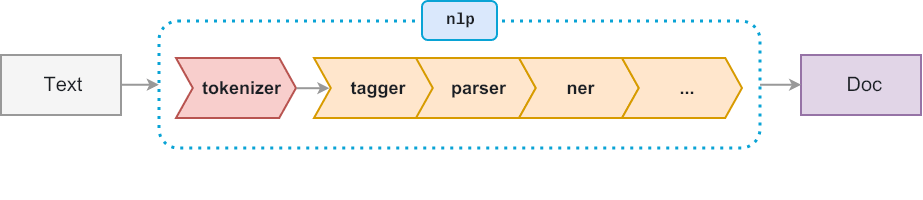
\includegraphics[width=0.8\linewidth,keepaspectratio]{spacy5}
\end{center}
	
{\tiny (Ref: https://spacy.io/usage/spacy-101)}
\end{frame}

%%%%%%%%%%%%%%%%%%%%%%%%%%%%%%%%%%%%%%%%%%%%%%%%%%%%%%%%%%%%%%%%%%%%%%%%%%%%%%%%%%
\begin{frame}[fragile]\frametitle{Tokenization}

\begin{lstlisting}
import spacy
nlp = spacy.load('en_core_web_sm')
text = 'Apple is looking for buying a U.K. startup for $1 billion'
doc = nlp(text)
for token in doc:
    print(token.text)
		
Apple
is
looking
for
buying
a
U.K.
startup
for
$
1
billion
\end{lstlisting}
	
{\tiny (Ref: https://spacy.io/usage/spacy-101)}
\end{frame}


%%%%%%%%%%%%%%%%%%%%%%%%%%%%%%%%%%%%%%%%%%%%%%%%%%%%%%%%%%%%%%%%%%%%%%%%%%%%%%%%%%
\begin{frame}[fragile]\frametitle{Sentence Segmentation}

\begin{lstlisting}
text = 'Apple is looking for buying a U.K. startup. Government has given permission.'

doc = nlp(text)
for sent in doc.sents:
    print(sent)
		
Apple is looking for buying a U.K. startup.
Government has given permission.
\end{lstlisting}
	
{\tiny (Ref: https://spacy.io/usage/spacy-101)}
\end{frame}

%%%%%%%%%%%%%%%%%%%%%%%%%%%%%%%%%%%%%%%%%%%%%%%%%%%%%%%%%%%%%%%%%%%%%%%%%%%%%%%%%%
\begin{frame}[fragile]\frametitle{Parts of Speech [POS] Tagging }

\begin{lstlisting}
print(doc)

>> Apple is looking for buying a U.K. startup for $1 billion

for token in doc:
    print(token.text, token.pos_)

Apple PROPN
is AUX
looking VERB
for ADP
buying VERB
a DET
U.K. PROPN
startup NOUN
for ADP
$ SYM
1 NUM
billion NUM
\end{lstlisting}
	
{\tiny (Ref: https://spacy.io/usage/spacy-101)}
\end{frame}

%%%%%%%%%%%%%%%%%%%%%%%%%%%%%%%%%%%%%%%%%%%%%%%%%%%%%%%%%%%%%%%%%%%%%%%%%%%%%%%%%%
\begin{frame}[fragile]\frametitle{Named Entity Recognition NER}

\begin{lstlisting}
print(doc)

>> Apple is looking for buying a U.K. startup for $1 billion

for token in doc:
    print(token.text, token.label_)

Apple ORG
U.K. GPE
$1 billion MONEY

doc = nlp('Apple is looking for buying a UK startup for $1 billion in 2020')
displacy.render(doc, style = 'ent')
\end{lstlisting}

\begin{center}
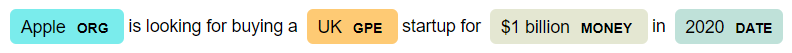
\includegraphics[width=0.8\linewidth,keepaspectratio]{spacy6}
\end{center}

{\tiny (Ref: https://spacy.io/usage/spacy-101)}
\end{frame}

%%%%%%%%%%%%%%%%%%%%%%%%%%%%%%%%%%%%%%%%%%%%%%%%%%%%%%%%%%%%%%%%%%%%%%%%%%%%%%%%%%
\begin{frame}[fragile]\frametitle{Sentence Segmentation}

\begin{lstlisting}
text = 'Apple is looking for buying a U.K. startup. Government has given permission.'

doc = nlp(text)
for sent in doc.sents:
    print(sent)
		
Apple is looking for buying a U.K. startup.
Government has given permission.
\end{lstlisting}
	
{\tiny (Ref: https://spacy.io/usage/spacy-101)}
\end{frame}

%%%%%%%%%%%%%%%%%%%%%%%%%%%%%%%%%%%%%%%%%%%%%%%%%%%%%%%%%%%%%%%%%%%%%%%%%%%%%%%%%%
\begin{frame}[fragile]\frametitle{Phrase Matching }

  \begin{itemize}
    \item Like Regular Expressions
		\item Rule-based matcher engines and components can find words and phrases
		\item Can give access to the tokens within the document and their relationships.
		\item Can easily access and analyze the surrounding tokens, merge spans into single tokens or add entries to the named entities in doc.ents.
  \end{itemize}
	
{\tiny (Ref: https://spacy.io/usage/spacy-101)}
\end{frame}

%%%%%%%%%%%%%%%%%%%%%%%%%%%%%%%%%%%%%%%%%%%%%%%%%%%%%%%%%%%%%%%%%%%%%%%%%%%%%%%%%%
\begin{frame}[fragile]\frametitle{Token-based matching }

  \begin{itemize}
    \item `Matcher' rules can refer to token annotations (e.g. the token text or tag\_, and flags (e.g. IS\_PUNCT).
		\item Lets you pass in a custom callback to act on matches – for example, to merge entities and apply custom labels
		\item To match large terminology lists, use the PhraseMatcher, which accepts Doc objects as match patterns
		\item Sample pattern \lstinline|[{"LOWER": "hello"}, {"IS_PUNCT": True}, {"LOWER": "world"}]|
  \begin{itemize}
    \item A token whose lowercase form matches “hello”, e.g. “Hello” or “HELLO”.
    \item A token whose is\_punct flag is set to True, i.e. any punctuation.
    \item A token whose lowercase form matches “world”, e.g. “World” or “WORLD”.
  \end{itemize}		
  \end{itemize}
	
{\tiny (Ref: https://spacy.io/usage/spacy-101)}
\end{frame}


%%%%%%%%%%%%%%%%%%%%%%%%%%%%%%%%%%%%%%%%%%%%%%%%%%%%%%%%%%%%%%%%%%%%%%%%%%%%%%%%%%
\begin{frame}[fragile]\frametitle{Token-based matching }

\begin{lstlisting}
from spacy.matcher import Matcher
from spacy.tokens import Span
text = 'Hello, world! hello world'
doc = nlp(text)

pattern = [{'LOWER': 'hello'}, {'IS_PUNCT': True, 'OP': '?'}, {'LOWER': 'world'}]
matcher = Matcher(nlp.vocab)
matcher.add('hw', None, pattern)
matches = matcher(doc)
print(macthes)
[(17790654416186116455, 0, 3), (17790654416186116455, 4, 6)]

for match_id, start, end in matches:
    string_id = nlp.vocab.strings[match_id]
    span = doc[start:end]
    print(match_id, string_id, start, end, span.text)
		
17790654416186116455 hw 0 3 Hello, world
17790654416186116455 hw 4 6 hello world		
\end{lstlisting}
	
{\tiny (Ref: https://spacy.io/usage/spacy-101)}
\end{frame}